\section{Results}
% Answer research questions

\subsection{The need for Distributed Machine Learning}
\subsubsection{Alternatives to Distributed Machine Learning}
\paragraph{Long-term sustainability}










\subsection{Underlying technology}
To give you an overview of how Distributed Machine Learning works, we'll give you an abstract framework that includes everything a real implementation should include. We do that by exploiting the three unique properties of Distributed Machine Learning, namely error tolerance, dynamic structural dependency and non-uniform convergence.\cite{Xing16}\\
Our goals include (1) to list regular Machine Learning algorithms that are commonly used in a distributed setting; (2) to find algorithms to determine the best parameters for the former algorithms; (3) to trade-off computation time with communication and accuracy; and (4) to minimize the amount of bits sent over the network so that the system is no bottlenecked by scarce network bandwidth.\\
Designing a general system in such a way that the regular Machine Learning algorithms can be distributed efficiently is challenging, because every algorithm has its own communication patterns \cite{Jia14}\cite{Newman09}\cite{Rich13}\cite{Smola10}\cite{Takac13}\cite{Tsi12}.

\subsubsection{Machine Learning algorithms}
We'll first look at Machine Learning is done at a single machine before looking at distributing these. We'll only give a brief description of the algorithms because single-node machine learning is not the focus of this paper.


\paragraph{Overview}
Machine Learning algorithm-families that are used in the literature and perform the actual "learning" include:
\begin{itemize}
	\item Graphical models \cite{Wain08}\cite{Kol09}\cite{Xin16}
	\begin{itemize}
		\item Latent Dirichlet Allocation Topic Model \cite{Blei03}
	\end{itemize}
	\item Regularized Bayesian models \cite{Zhu09}\cite{Zhu09-2}\cite{Zhu14}
	\item Nonparametric Bayesian models \cite{Grif05}\cite{Teh06}
	\item Sparse structured models
	\begin{itemize}
		\item Lasso regression (group Lasso)
	\end{itemize}
	\item Large-margin methods
	\item Deep learning
	\item Matrix factorization
	\item Sparse coding
	\item Latent space modeling
	\item Distance metric learning
	\item Non-negative matrix factorization
	\item Principal component analysis
\end{itemize}


\paragraph{Algorithms to find best parameters}
To find the parameters for these algorithms we can use several Machine Learning workhorse implementations that can be re-used across different Machine Learning algorithm-families. These include:
\begin{itemize}
	\item First-order techniques
	\begin{itemize}
		\item Stochastic gradient descent
		\item Stochastic dual coordinate ascent\cite{Shal13}
		\item L-BFGS
		\item Conjugate gradient
	\end{itemize}
	\item Second-order techniques
	\begin{itemize}
		\item Newton descent
		\item Quasi-Newton descent
	\end{itemize}
	\item Coordinate descent
	\item Markov-Chain Monte-Carlo
	\item Variational inference
\end{itemize}


% --------


\subsubsection{Partitioning and distribution algorithms}
Now we'll look the abstraction of the general design for a distributed Machine Learning operating system that executes the Machine Learning workhorses across a wide variety of hardware.


\paragraph{Computation time vs communication vs accuracy}


\paragraph{Scheduling and balancing the workloads}
There are 3 things to take into account when partitioning an ML program in order to parallelize it:\cite{Xing16}\\
\begin{enumerate}
	\item Deciding which tasks go or don' go together in parallel
	\item Deciding the order in which tasks will be executed
	\item Ensuring an even load distribution across the machines
\end{enumerate}


\paragraph{Bridging computation and communication}
Let's look at several ways to efficiently communicate between the nodes taking the interleaving of parallel program computations and inter-worker communication into account.
\begin{enumerate}
	\item \underline{BSP:} Bulk Synchronous Parallel, the most simple model; programs will alternate between a computation and a communication phase to ensure consistency\cite{Xing16}. An example of program following the BSP bridging model is MapReduce.\\
	An advantage is that serializable BSP ML programs are guaranteed to output a correct solution. A disadvantage is that finished workers must wait at every synchronization barrier till the other works are finished, which results in overhead\cite{Chilimbi14}. Another disadvantage is that the synchronization barrier may take a significant amount of time, because of slow communication between the workers.
	\item \underline{SSP:} Stale Synchronous Parallel, allows the fastest worker to be ahead of the slowest worker up to a bounded number of iterations before the workers are stopped. The fast workers may work for a while on state data, but SSP still limits the maximum staleness between any pair of workers. An advantage is that it still enjoys strong model convergence guarantees. A disadvantage is that, when machines temporarily slow down due to other tasks or users and cause large staleness, the convergence rates are poor.
	\item \underline{ASP:} Approximate Synchronous Parallel, limits how inaccurate a parameter can be, in contrast to SSP that limits how stale a parameter can be. An advantage is that, when an aggregated update is insignificant, then the server can delay synchronization indefinitely. A disadvantage is that it can be hard to choose the parameter that defines which update are significant and which are not. \cite{Hsieh17}
	\item \underline{BAP / TAP:} Barrierless Asynchronous Parallel\cite{Han15} or Total Asynchronous Parallel\cite{Hsieh17}; worker machines communicate in parallel without waiting for each other. The advantage is that it usually obtains the highest speedup possible. A disadvantage is that the model converges slowly or even incorrectly because the error grows with the delay, unlike BSP and SSP. \cite{Han15}
\end{enumerate}
At the moment, ASP is the state-of-the-art method.


\paragraph{Communication strategies}
To distribute Machine Learning algorithms we can choose to partition either the data or the model across the machines - referred to respectively as data parallelism and model parallelism \cite{Die12}. These two types of parallelism can be applied at the same time \cite{Xing16}. Data parallelism can be applied to every ML algorithm with an i.i.d. assumption over the data samples, which are most ML algorithms \cite{Xing16}. It partitions the data and assigns it to parallel machines. Model parallelism cannot be applied to most ML algorithms, because the model parameters generally don't have this i.i.d. assumption. It partitions the model parameters and assigns that to parallel machines.\\
There are several communication management strategies\cite{Xing16} used to spread and reduce the amount of data communicated between machines:
\begin{itemize}
	\item To prevent bursts of communication over the network, for example after a mapper is finished, continuous communication is used, for example in the state-of-the-art implementation Bösen\cite{Wei15}.
	
	\item Neural networks are composed out of layers, of which the training by using the back-propagation gradient descent algorithm is highly sequential. Because the top layers of neural networks contain a lot more parameters while it accounts only for a small part of the total computation \cite{Xing16}, WFBP \cite{Zhang17} was proposed to spread the computation and communication out in an optimal fashion.
	
	\item Hybrid communication (HybComm) Because WBFP does not reduce the communication overhead, HybComm \cite{Zhang17} was proposed. Effectively it combines Parameter Servers (PS)\cite{Wei15} with Sufficient Factor Broadcasting (SFB)\cite{Xie15} by being aware of both the mathematical property of neural networks and the structure of computing clusters. See below for more information about PS and SFB.
	
\end{itemize}


\paragraph{Network topologies}
There are several network topologies used for Distributed Machine Learning clusters:
\begin{itemize}
	\item \textbf{Trees} AllReduce\cite{Agar14}
	\item \textbf{Centralized storage} Parameter Server (PS)\cite{Agar14}
	\item \textbf{Decentralized storage} e.g. peer-to-peer storage (e.g. Sufficient Factor Broadcasting (SFB)\cite{Li13})
\end{itemize}










\subsection{Currently used implementations}
\subsubsection{Generic distributed system frameworks}
Distributed system have already been implemented in the industry to solve the problem of companies possessing massive amounts of data that they want to be able to query and analyze. These frameworks largely rely on the fact that it is cheaper
to have multiple servers, each of them with a relatively small storage capacity and computing power, rather than having one expensive large server.

\paragraph{The frameworks}
The basis of existing frameworks is based on the Google File System\cite{Ghem03}. The \textit{Google File System} or \textit{GFS} is the system that is used within Google to handle all the Big data needs within the company. It splits all the data that is uploaded to the cluster up into chunks, which are then split over the "chunk servers" in the node, and replicated a predefined number of times (usually 3) in order to guarantee that the data is not lost when a server fails. The
data on the chunk servers can then be accessed by a user by contacting the master, which knows exactly on which servers each chunk is saved.\cite{Ghem03} The data and work-flow is described in figure \ref{GFS_Architecture} below.

\begin{figure}
  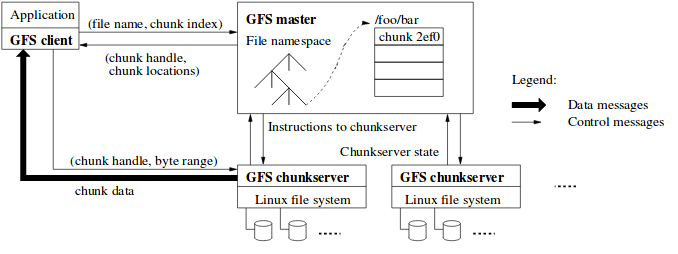
\includegraphics[width=\textwidth]{GFS_Architecture.png}
  \caption{Google File System architecture\cite{Ghem03}}
  \label{GFS_Architecture}
\end{figure}

The GFS architecture that was described in its paper by Google was adapted into an open-source solution called Hadoop \cite{Shv10}. Hadoop was developed mainly by Yahoo!, distributed as an Apache project and functions essentially the same as GFS. There are only minor differences with GFS such as the naming of certain entities and the chunk size. A typical use case of adding a file to the Hadoop File System (HDFS) is show in figure \ref{Hadoop_usecase} below.

\begin{figure}
  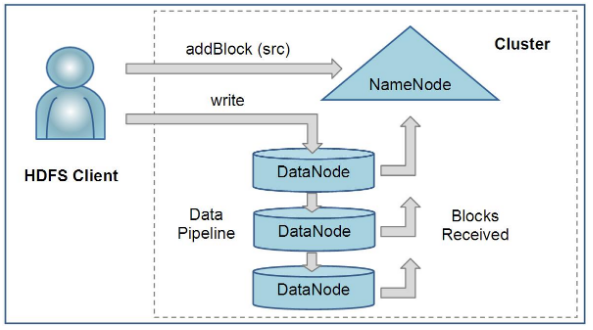
\includegraphics[width=\textwidth]{Hadoop_use_case.png}
  \caption{The data flow when adding a file to the HDFS\cite{Shv10}}
  \label{Hadoop_usecase}
\end{figure}

\paragraph{Uses of the frameworks}
The storage framework highlighted above, is the most-common file-system that empower Big Data implementations today. These implementations are frameworks such as MapReduce and the Apache Spark engine.

\paragraph{MapReduce}
MapReduce is a new framework for processing data and was developed by Google\cite{Dean04} in order to process data in a distributed setting. Firstly, in the \textit{map phase} all data is split into tuples (called key-value pairs). Then, during the shuffle phase, these key-value pairs are shuffled and passed to the \textit{reduce phase} in which a calculation (often an aggregation) is performed on them to generate the a single output value. The main benefit of this framework is that the data can be distributed across a large amount of machines (which are using for example GFS or HDFS). Additionally, instead of communicating the data between the nodes, the program is communicated between the nodes which is magnitudes smaller and more efficient to pass around. A general overview of the execution of a map-reduce problem is given in figure \ref{mapreduce_execution}.

\begin{figure}
  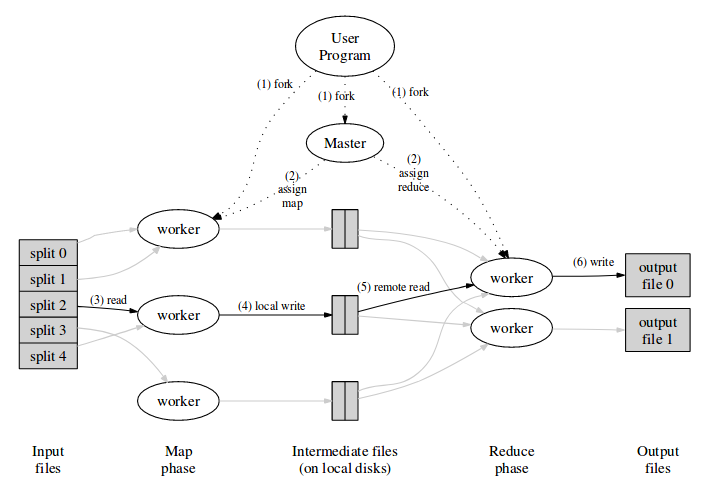
\includegraphics[width=\textwidth]{mapreduce_execution.png}
  \caption{Overview of the execution of a mapreduce problem\cite{Dean04}}
  \label{mapreduce_execution}
\end{figure}

Furthermore the MapReduce framework is similar to the \textit{Bulk-Synchronous processing (BSP)} style which is a little older. However, there are some differences as the MapReduce framework does not allow communication between nodes in the map phase, but only allows communication during the shuffle phase, in-between the mapping and reduce phase\cite{Pace12}.\\
Since BSP and Map-reduce are so similar, peope have worked on transforming BSP tasks into MapReduce tasks. Goodrich et al.\cite{Goo11} has shown that all BSP programs can be converted into MapReduce programs and other researchers have gone as far as to say that all MapReduce task are so similar to BSP tasks that, because BSP has a more theoretical basis, all tasks should be modeled as BSP tasks but implemented using the Map-reduce framework in order to gain the speed of MapReduce and the correctness of BSP\cite{Pace12}.

\paragraph{Apache Spark}
Like MapReduce, Apache Spark is another service built on top of a distributed file system to run programs on a distributed dataset. Spark is an open-source cluster-computing framework that is capable of executing an entire directed acyclic graph of transformations (like mappings) and actions (like reductions) fully in memory\cite{Sparkwebsite}. This is contrast to MapReduce, that forces the programmer to first use a mapping phase and then a reduce phase. This way, Spark is a lot faster than MapReduce because when, for example, 2 mapping phases are needed, 2 MapReduce tasks need to be executed which both require to write all (intermediate) data to the disk. Spark on the other hand can keep all the data in-memory which saves expensive writes to the disk, but needs to take additional steps to prevent losing processed data when there's a power outage.\\

The way in which Spark solves this problem is by using \textbf{RDDs} (Resilient Distributed Datasets). These datasets are read-only and new ones can only be created from data stored on the disk, or transforming existing RDDs\cite{Zaha12}. The Resilient part comes into play when the data is lost. Each RDD has a lineage graph, which shows what transformations have been executed on it. This means that once some data is lost, Spark can trace the path that RDD has followed by using the lineage graph and recalculate any lost data. It is important that the lineage graph does not contain any cycles, i.e. is a Directed Acylic Graph (DAG), because otherwise the data cannot be recovered as Spark will run into an infinite loop.

\begin{figure}
  \begin{center}
    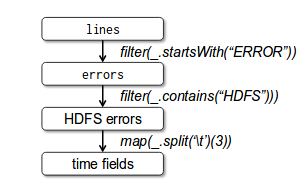
\includegraphics[scale=0.5]{Lineage_graph.png}
  \end{center}
  \caption{Example of the lineage graph of an RDD\cite{Zaha12}}
  \label{lineagegraph}
\end{figure}

\subsubsection{Domain-specific implementations}
\subsubsection{Current challenges}










\subsection{Privacy challenges}
